\documentclass[aspectratio=169,11pt]{beamer}

% ---- Minimalist theme ----
\usetheme{default}
\usecolortheme{default}
\setbeamertemplate{navigation symbols}{}
\setbeamertemplate{frametitle continuation}{}
\setbeamertemplate{itemize items}[circle]
\setbeamertemplate{enumerate items}[default]

% ---- Font: TeX Gyre Heros ----
\usepackage[T1]{fontenc}
\usepackage{tgheros}
\renewcommand{\familydefault}{\sfdefault}
\usepackage{microtype}

% ---- Packages ----
\usepackage{amsmath}
\usepackage{booktabs}
\usepackage{array}
\usepackage{tikz}
\usepackage{xcolor}
\usepackage{hyperref}
\usetikzlibrary{arrows.meta,positioning,calc,fit}

% ---- Maastricht University colors ----
\definecolor{umdark}{HTML}{001C3D}
\definecolor{umorange}{HTML}{E84E10}
\definecolor{umlight}{HTML}{4A90C4}
\definecolor{umgray}{HTML}{6B7280}
\definecolor{umbg}{HTML}{F8F9FA}
\definecolor{umfaint}{HTML}{E5E7EB}
\newcommand{\icite}[1]{{\footnotesize\color{umgray!85}#1}}

% ---- Apply colors to Beamer ----
\setbeamercolor{normal text}{fg=umdark}
\setbeamercolor{frametitle}{fg=umdark}
\setbeamercolor{title}{fg=umdark}
\setbeamercolor{subtitle}{fg=umgray}
\setbeamercolor{author}{fg=umgray}
\setbeamercolor{date}{fg=umgray}
\setbeamercolor{institute}{fg=umorange}
\setbeamercolor{itemize item}{fg=umorange}
\setbeamercolor{itemize subitem}{fg=umlight}
\setbeamercolor{enumerate item}{fg=umorange}
\setbeamercolor{block title}{bg=umdark,fg=white}
\setbeamercolor{block body}{bg=umdark!5,fg=umdark}
\setbeamercolor{block title alerted}{bg=umorange,fg=white}
\setbeamercolor{block body alerted}{bg=umorange!8,fg=umdark}
\setbeamercolor{block title example}{bg=umlight,fg=white}
\setbeamercolor{block body example}{bg=umlight!8,fg=umdark}

% ---- Frametitle style ----
\setbeamertemplate{frametitle}{%
  \vspace{0.35cm}%
  \noindent\hspace*{0pt}%
  \parbox{\textwidth}{%
    {\usebeamerfont{frametitle}\usebeamercolor[fg]{frametitle}\insertframetitle}%
    \vspace{2pt}\\%
    {\color{umorange}\rule{\textwidth}{1.2pt}}%
  }%
  \vspace{-2pt}%
}
\setbeamerfont{frametitle}{size=\large,series=\bfseries}
\setbeamersize{text margin left=0.7cm,text margin right=0.7cm}

% ---- Footline ----
\setbeamertemplate{footline}{%
  \hbox{%
    \begin{beamercolorbox}[wd=\paperwidth,ht=2.2ex,dp=1ex]{footline}%
      \hspace{1em}{\scriptsize\color{umgray}Midway Proposal -- Carrier Origin and Steganographic Detectability}%
      \hfill%
      {\scriptsize\color{umgray}\insertframenumber/\inserttotalframenumber}%
      \hspace{1em}%
    \end{beamercolorbox}%
  }%
}

% ---- Metadata ----
\title{Does the Source of Carrier Image Affect\\Steganographic Detectability?}
\subtitle{Full Midway Proposal}
\newcommand{\teamauthors}{Abdul Moiz Akbar \;|\; Malo Coquin \;|\; Daria Gjonbalaj \;|\; Nico Muller-Spath\\Jimena Narvaez del Cid \;|\; David Wicker \;|\; Nikolas Zouros}
\author[Project 2.2 Team]{Project 2.2 Team}
\institute{Department of Advanced Computing Sciences\\Maastricht University}
\date{Project 2.2 \;|\; February 2026}

\begin{document}

% ============================================================
% Title
% ============================================================
\begin{frame}[plain]
\vfill
\begin{center}
{\color{umorange}\rule{0.42\textwidth}{2pt}}\\[12pt]
{\LARGE\bfseries\color{umdark}\inserttitle}\\[10pt]
{\normalsize\color{umgray}\insertsubtitle}\\[16pt]
{\small\color{umdark}\teamauthors}\\[8pt]
{\small\color{umorange}\insertinstitute}\\[8pt]
{\footnotesize\color{umgray}\insertdate}\\[12pt]
{\color{umorange}\rule{0.42\textwidth}{2pt}}
\end{center}
\vfill
\end{frame}

% ============================================================
\begin{frame}{Agenda}
\begin{columns}[T]
\begin{column}{0.47\textwidth}
\begin{enumerate}
\item Motivation and problem statement
\item Research questions and verification
\item Chosen approaches
\item Experiments and validation
\end{enumerate}
\end{column}
\begin{column}{0.47\textwidth}
\begin{enumerate}
\setcounter{enumi}{4}
\item Prototype status
\item Related work positioning
\item Relation to curriculum
\item Planning and passing requirements
\end{enumerate}
\end{column}
\end{columns}
\end{frame}

% ============================================================
\section{Motivation}
% ============================================================
\begin{frame}{Motivation and Problem Statement}
\begin{columns}[T]
\begin{column}{0.56\textwidth}
\small
\begin{itemize}
\item Image steganography detectability depends on carrier statistics, not only embedding logic \icite{(Petitcolas et al., 1999; Cheddad et al., 2010; Fridrich \& Kodovsky, 2012).}
\item Most steganalysis benchmarks assume camera photos with familiar noise/compression traces.
\item Modern generators (Stable Diffusion, StyleGAN3) produce photorealistic images from different processes \icite{(Rombach et al., 2022; Karras et al., 2021).}
\item Synthetic images have measurable statistical fingerprints that may alter detector behavior \icite{(Wang et al., 2020; Corvi et al., 2023).}
\end{itemize}
\end{column}
\begin{column}{0.40\textwidth}
\begin{alertblock}{Central Problem}
\small
Do steganalysis methods designed and validated on photographs remain effective when the carrier is ML-generated?
\end{alertblock}

\begin{block}{Closest prior work}
\small
\icite{De et al. (2022)} show AI-generated image steganography, but not a controlled real-vs-ML comparison with standardized LSB/DCT detectors.
\end{block}
\end{column}
\end{columns}
\end{frame}

\begin{frame}{Why This Study Matters}
\begin{columns}[T]
\begin{column}{0.32\textwidth}
\begin{block}{Security}
\small
\begin{itemize}
\item If synthetic carriers are harder to detect, attackers gain an easy evasion path.
\item If easier, defenders get a concrete screening advantage.
\end{itemize}
\end{block}
\end{column}
\begin{column}{0.32\textwidth}
\begin{block}{Scientific gap}
\small
\begin{itemize}
\item Interaction between generative-model distributions and embedding distortion is largely unexplored.
\item Need controlled experiments isolating carrier origin.
\end{itemize}
\end{block}
\end{column}
\begin{column}{0.32\textwidth}
\begin{block}{Practical relevance}
\small
\begin{itemize}
\item AI images are now common in social and communication channels.
\item Practitioners need evidence on retraining/adaptation requirements.
\end{itemize}
\end{block}
\end{column}
\end{columns}
\vspace{0.15cm}
{\small\color{umgray}\textbf{Study scope:} 2 x 2 x 3 x 2 factorial design over 1,000 images, with CPU-feasible execution in 7 weeks.}
\end{frame}

% ============================================================
\section{Research Questions}
% ============================================================
\begin{frame}{Research Questions}
\scriptsize
\begin{columns}[T]
\begin{column}{0.49\textwidth}
\begin{block}{RQ1: Carrier origin}
Does carrier-image origin (real vs ML-generated) affect detectability under identical settings?
\end{block}
\begin{block}{RQ2: Payload}
Does increasing payload size widen the real-vs-ML detectability gap?
\end{block}
\begin{block}{RQ3: Encryption}
Does encrypting payload before embedding change detectability, and does origin modify that effect?
\end{block}
\end{column}
\begin{column}{0.49\textwidth}
\begin{block}{RQ4: Embedding method}
Do LSB and DCT interact differently with carrier origin in terms of detectability?
\end{block}
\begin{block}{RQ5: Image quality}
How are PSNR/SSIM/FSIM affected by embedding method and payload size?
\end{block}
\end{column}
\end{columns}
\end{frame}

\begin{frame}{Verification Criteria by RQ}
\scriptsize
\renewcommand{\arraystretch}{1.2}
\begin{tabular}{@{}p{0.9cm}p{7.4cm}p{4.2cm}@{}}
\toprule
\textbf{RQ} & \textbf{Verification target} & \textbf{Primary analysis} \\
\midrule
RQ1 & Real-vs-ML AUC difference with fixed settings. & RS and SRM+FLD + significance/effect size \\
RQ2 & AUC-gap trend across Low/Medium/High payload. & Trend test + carrier$\times$payload interaction \\
RQ3 & Plain vs AES-256-CBC detectability difference. & Condition-wise AUC comparisons by method and origin \\
RQ4 & Carrier-origin dependence on LSB vs DCT. & Two-way ANOVA interaction term \\
RQ5 & Quality stability across conditions. & PSNR/SSIM/FSIM against target thresholds \\
\bottomrule
\end{tabular}
\vspace{0.2cm}
\begin{exampleblock}{Common statistical settings}
\small
We evaluate performance primarily with ROC-AUC and report uncertainty and effect size alongside significance, using a stricter threshold to account for multiple comparisons.
\end{exampleblock}
\end{frame}

\begin{frame}{Hypotheses and Decision Criteria}
\scriptsize
\begin{columns}[T]
\begin{column}{0.49\textwidth}
\begin{block}{RQ1 (Carrier Origin)}
\textbf{H1:} Carrier origin affects RS-detected AUC.\\
\textit{Test:} Wilcoxon (RS) + effect size.\\
\textbf{H2:} Carrier origin affects SRM+FLD-detected AUC.\\
\textit{Test:} Wilcoxon (SRM+FLD) + effect size.
\end{block}

\begin{block}{RQ2 (Payload)}
\textbf{H3:} Real-vs-ML AUC gap increases with payload.\\
\textit{Test:} Spearman trend + carrier$\times$payload interaction.
\end{block}
\end{column}

\begin{column}{0.49\textwidth}
\begin{block}{RQ3 (Encryption)}
\textbf{H4:} AES-256 payload encryption changes AUC vs plain.\\
\textit{Test:} Wilcoxon by condition (plain vs AES).\\
\textbf{H5:} Encryption effect differs by carrier origin.\\
\textit{Test:} Encryption$\times$carrier interaction.
\end{block}

\begin{block}{RQ4 (Embedding Method)}
\textbf{H6:} LSB-vs-DCT effect depends on carrier origin.\\
\textit{Test:} Two-way ANOVA interaction.
\end{block}
\end{column}
\end{columns}
{\scriptsize\color{umgray}Primary metric: ROC-AUC. Report significance, uncertainty intervals, and effect size. Bonferroni across six confirmatory hypotheses: $\alpha_{\text{adj}} = 0.05/6 \approx 0.0083$.}
\end{frame}

\begin{frame}{End-to-End Experimental Pipeline}
\centering
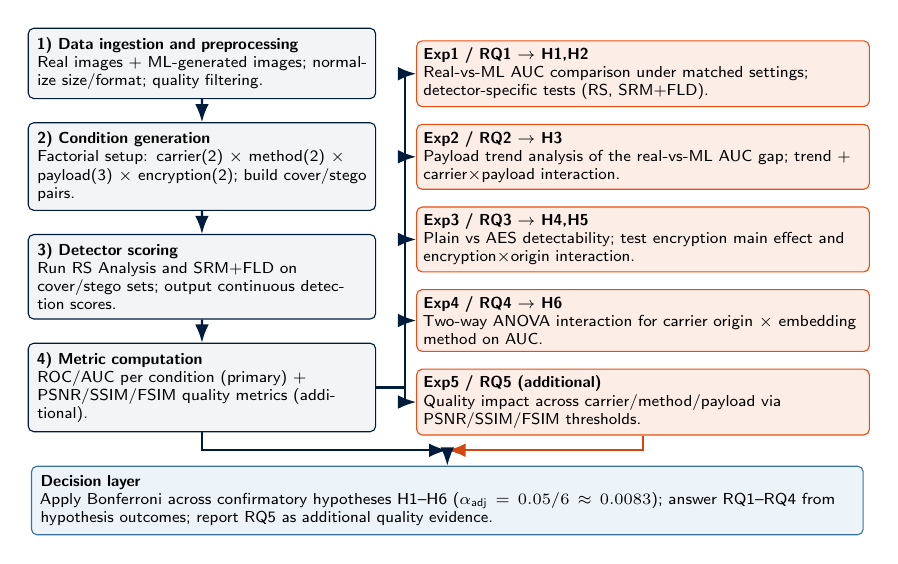
\begin{tikzpicture}[
  >=Latex,
  scale=0.82,
  transform shape,
  node distance=3.6mm and 5.2mm,
  every node/.style={font=\scriptsize},
  pstep/.style={draw=umdark,rounded corners=2pt,fill=umdark!5,align=left,inner sep=4pt,text width=5.1cm},
  pexp/.style={draw=umorange,rounded corners=2pt,fill=umorange!10,align=left,inner sep=3pt,text width=6.8cm},
  pnote/.style={draw=umlight!80!black,rounded corners=2pt,fill=umlight!10,align=left,inner sep=4pt,text width=12.6cm}
]
\node[pstep] (s1) {\textbf{1) Data ingestion and preprocessing}\\Real images + ML-generated images; normalize size/format; quality filtering.};
\node[pstep,below=of s1] (s2) {\textbf{2) Condition generation}\\Factorial setup: carrier(2) $\times$ method(2) $\times$ payload(3) $\times$ encryption(2); build cover/stego pairs.};
\node[pstep,below=of s2] (s3) {\textbf{3) Detector scoring}\\Run RS Analysis and SRM+FLD on cover/stego sets; output continuous detection scores.};
\node[pstep,below=of s3] (s4) {\textbf{4) Metric computation}\\ROC/AUC per condition (primary) + PSNR/SSIM/FSIM quality metrics (additional).};

\node[pexp,right=6.2mm of s1,yshift=-1.6mm] (e1) {\textbf{Exp1 / RQ1 $\rightarrow$ H1,H2}\\Real-vs-ML AUC comparison under matched settings; detector-specific tests (RS, SRM+FLD).};
\node[pexp,below=2.6mm of e1] (e2) {\textbf{Exp2 / RQ2 $\rightarrow$ H3}\\Payload trend analysis of the real-vs-ML AUC gap; trend + carrier$\times$payload interaction.};
\node[pexp,below=2.6mm of e2] (e3) {\textbf{Exp3 / RQ3 $\rightarrow$ H4,H5}\\Plain vs AES detectability; test encryption main effect and encryption$\times$origin interaction.};
\node[pexp,below=2.6mm of e3] (e4) {\textbf{Exp4 / RQ4 $\rightarrow$ H6}\\Two-way ANOVA interaction for carrier origin $\times$ embedding method on AUC.};
\node[pexp,below=2.6mm of e4] (e5) {\textbf{Exp5 / RQ5 (additional)}\\Quality impact across carrier/method/payload via PSNR/SSIM/FSIM thresholds.};
\node[draw=none,fit=(e1)(e5),inner sep=0pt] (expgrp) {};

\node[pnote,below=5.2mm of s4,xshift=3.8cm] (d1) {\textbf{Decision layer}\\Apply Bonferroni across confirmatory hypotheses H1--H6 ($\alpha_{\text{adj}}=0.05/6\approx0.0083$); answer RQ1--RQ4 from hypothesis outcomes; report RQ5 as additional quality evidence.};
\coordinate (join) at ($(d1.north)+(0,2.4mm)$);

\draw[->,thick,umdark] (s1) -- (s2);
\draw[->,thick,umdark] (s2) -- (s3);
\draw[->,thick,umdark] (s3) -- (s4);
\draw[->,thick,umdark] (s4.east) -- ++(0.45,0) |- (e1.west);
\draw[->,thick,umdark] (s4.east) -- ++(0.45,0) |- (e2.west);
\draw[->,thick,umdark] (s4.east) -- ++(0.45,0) |- (e3.west);
\draw[->,thick,umdark] (s4.east) -- ++(0.45,0) |- (e4.west);
\draw[->,thick,umdark] (s4.east) -- ++(0.45,0) |- (e5.west);
\draw[->,thick,umdark] (s4.south) |- (join);
\draw[->,thick,umorange!90!black] (expgrp.south) |- (join);
\draw[->,thick,umdark] (join) -- (d1.north);
\end{tikzpicture}
\end{frame}

% ============================================================
\section{Chosen Approaches}
% ============================================================
\begin{frame}{Chosen Approach: Factorial Design and Conditions}
\begin{columns}[T]
\begin{column}{0.52\textwidth}
\begin{block}{Design matrix}
\small
\begin{itemize}
\item \textbf{Carrier type (2):} Real, ML-generated
\item \textbf{Embedding (2):} Spatial LSB, frequency-domain DCT-QIM
\item \textbf{Payload (3):} Low, Medium, High
\item \textbf{Detectors (2 main):} RS Analysis, SRM+FLD
\end{itemize}
\end{block}
\end{column}
\begin{column}{0.44\textwidth}
\begin{alertblock}{Sample size}
\small
\begin{itemize}
\item 500 real images
\item 500 ML-generated images
\item 1,000 total carriers
\item Full condition coverage
\end{itemize}
\end{alertblock}
\end{column}
\end{columns}
\vspace{0.1cm}
\begin{exampleblock}{Controlled variable principle}
\small
Carrier origin is treated as the central independent variable; image size/format, embedding pipelines, payload levels, and detector protocols are standardized across conditions.
\end{exampleblock}
\end{frame}

\begin{frame}{Datasets and Preprocessing}
\small
\begin{columns}[T]
\begin{column}{0.48\textwidth}
\begin{block}{Real photographs (500)}
\begin{itemize}
\item RAISE: 250 images (RAW-derived forensic-quality baseline)
\item COCO: 150 images
\item Flickr30k: 100 images
\end{itemize}
\vspace{0.1cm}
\icite{Sources: Dang-Nguyen et al. (2015), Lin et al. (2014), Young et al. (2014)}
\end{block}
\end{column}
\begin{column}{0.48\textwidth}
\begin{block}{ML-generated images (500)}
\begin{itemize}
\item Stable Diffusion v2.1: 250 images
\item StyleGAN3: 250 images
\item Prompts aligned to COCO/Flickr semantics
\end{itemize}
\vspace{0.1cm}
\icite{Sources: Rombach et al. (2022), Karras et al. (2021)}
\end{block}
\end{column}
\end{columns}

\begin{alertblock}{Normalization and quality gate}
\small
All images normalized to 512x512 RGB 8-bit PNG. BRISQUE <= 50 filter for generated outputs to exclude low-quality artifacts.
\end{alertblock}
\end{frame}

\begin{frame}{Embedding Methods}
\begin{columns}[T]
\begin{column}{0.49\textwidth}
\begin{block}{LSB substitution (spatial)}
\small
\begin{itemize}
\item PRNG-keyed pixel/channel selection
\item k = 1 for low and medium payload
\item k = 2 for high payload
\item Optional AES-256-CBC payload encryption
\end{itemize}
\end{block}
\end{column}
\begin{column}{0.49\textwidth}
\begin{block}{DCT-QIM (frequency)}
\small
\begin{itemize}
\item 8x8 block DCT per channel
\item Mid-frequency zigzag coefficients (10--54)
\item QIM embedding:
\[
C'_i = \Delta \cdot \mathrm{round}(C_i/\Delta) \pm \Delta/4
\]
\end{itemize}
\end{block}
\end{column}
\end{columns}
\begin{exampleblock}{Method rationale}
\small
LSB and DCT represent the two canonical embedding domains, allowing direct tests of method-origin interactions under controlled payload settings.
\end{exampleblock}
\end{frame}

\begin{frame}{Payload and Encryption Conditions}
\small
\renewcommand{\arraystretch}{1.2}
\begin{tabular}{@{}p{2.3cm}p{2.6cm}p{2.6cm}p{5.0cm}@{}}
\toprule
\textbf{Level} & \textbf{Approx. bpp} & \textbf{LSB setting} & \textbf{Purpose} \\
\midrule
Low & \(\approx 0.08\) & \(k=1\) sparse mask & Near-threshold detectability \\
Medium & \(\approx 0.16\) & \(k=1\) denser mask & Baseline operating point \\
High & \(\approx 0.32\) & \(k=2\) & Stress-test detector sensitivity \\
\bottomrule
\end{tabular}
\vspace{0.2cm}

\begin{columns}[T]
\begin{column}{0.49\textwidth}
\begin{block}{Encryption condition}
\small
Each payload level is tested in:
\begin{itemize}
\item Plain payload mode
\item AES-256-CBC pre-encrypted mode
\end{itemize}
\end{block}
\end{column}
\begin{column}{0.49\textwidth}
\begin{block}{Why include encryption?}
\small
It isolates whether message-bit structure contributes to detectability beyond carrier-level distortion.
\end{block}
\end{column}
\end{columns}
\end{frame}

\begin{frame}{Steganalysis Detectors and Validation Metrics}
\small
\begin{columns}[T]
\begin{column}{0.50\textwidth}
\begin{block}{Detector set}
\small
\begin{itemize}
\item \textbf{RS Analysis} (training-free statistical baseline)
\item \textbf{SRM+FLD} (feature-based classical ML detector)
\item \textbf{\(\chi^2\) attack} as supplementary LSB check
\end{itemize}
\vspace{0.05cm}
\icite{References: Fridrich et al. (2001), Westfeld and Pfitzmann (1999), Fridrich and Kodovsky (2012)}
\end{block}
\end{column}
\begin{column}{0.46\textwidth}
\begin{block}{Primary metrics}
\small
\begin{itemize}
\item ROC-AUC (primary)
\item Accuracy at Youden's J
\item Equal Error Rate
\item FPR at 5\% FNR
\end{itemize}
\end{block}
\end{column}
\end{columns}

\begin{exampleblock}{Statistical analysis plan}
\small
Two-way ANOVA (carrier x method; payload covariate), Wilcoxon pairwise tests, effect sizes, and Bonferroni-adjusted significance threshold.
\end{exampleblock}
\end{frame}

% ============================================================
\section{Experiments}
% ============================================================
\begin{frame}{Experiment Plan I (RQ1 and RQ2)}
\small
\begin{block}{Exp. 1 -- Carrier origin effect (RQ1)}
\begin{itemize}
\item Apply RS and SRM+FLD across all payload levels and methods.
\item Compare AUC for real vs ML-generated carriers.
\item Decide with Wilcoxon significance and effect size.
\end{itemize}
\end{block}

\begin{block}{Exp. 2 -- Payload sensitivity (RQ2)}
\begin{itemize}
\item Track real-vs-ML AUC gap across Low, Medium, High payload.
\item Test monotonic trend (Spearman) and carrier x payload interaction.
\item Decide whether payload amplifies origin-dependent detectability.
\end{itemize}
\end{block}
\end{frame}

\begin{frame}{Experiment Plan II (RQ3 and RQ4)}
\small
\begin{block}{Exp. 3 -- Encryption effect (RQ3)}
\begin{itemize}
\item Compare plain vs AES-encrypted payload AUC per carrier and method.
\item Test whether encryption effect differs by carrier origin.
\end{itemize}
\end{block}

\begin{block}{Exp. 4 -- Method interaction (RQ4)}
\begin{itemize}
\item Run two-way ANOVA on SRM AUC with carrier origin and method factors.
\item Confirm whether the detectability gap depends on LSB vs DCT.
\end{itemize}
\end{block}
\end{frame}

\begin{frame}{Experiment Plan III (RQ5)}
\small
\begin{block}{Exp. 5 -- Image quality (RQ5)}
\begin{itemize}
\item Compute PSNR, SSIM, and FSIM for each stego condition versus cover.
\item Check whether quality remains within target ranges across methods and payload levels.
\end{itemize}
\end{block}

\begin{alertblock}{Interpretation policy}
\small
Null findings remain valid outcomes; all major results reported with confidence intervals and effect sizes.
\end{alertblock}
\end{frame}

\begin{frame}{Complete ROC-AUC Output Set}
\scriptsize
\begin{columns}[T]
\begin{column}{0.49\textwidth}
\begin{block}{A) Per-condition ROC curve panels}
\begin{itemize}
\item Panel grid fixed by detector $\times$ method $\times$ payload $\times$ encryption; each panel overlays real vs ML ROC curves.
\item Count: $2\times2\times3\times2 = 24$ panels.
\end{itemize}
\end{block}

\begin{block}{B) Exp.2 payload-trend AUC-gap plots}
\begin{itemize}
\item Plot $\Delta$AUC = AUC(real) $-$ AUC(ML) over Low/Medium/High payload.
\item Count: $2\times2\times2 = 8$ plots.
\end{itemize}
\end{block}
\end{column}

\begin{column}{0.49\textwidth}
\begin{block}{C) Exp.3 encryption-effect AUC plots}
\begin{itemize}
\item Compare plain vs AES AUC values.
\item Count: $2\times2\times2 = 8$ plots.
\end{itemize}
\end{block}

\begin{block}{D) Exp.4 interaction plots}
\begin{itemize}
\item Primary: SRM interaction plot (method $\times$ origin) from ANOVA.
\item One pooled plot + six optional diagnostics stratified by payload $\times$ encryption.
\end{itemize}
\end{block}
\end{column}
\end{columns}
\vspace{-0.05cm}
\begin{exampleblock}{Inventory summary}
\scriptsize
Core ROC-AUC output set: $24 + 8 + 8 + 1 = 41$ figures (+6 optional diagnostics). RQ5 quality outputs (PSNR/SSIM/FSIM) are reported separately (not ROC-AUC).
\end{exampleblock}
\end{frame}

% ============================================================
\section{Prototype}
% ============================================================
\begin{frame}{Prototype Status}
\begin{columns}[T]
\begin{column}{0.49\textwidth}
\begin{block}{Vertical prototype (algorithm depth)}
\small
Core components validated on a small test subset:
\begin{itemize}
\item LSB embedding/extraction
\item DCT-QIM embedding
\item RS Analysis
\item SRM feature extraction/classification
\end{itemize}
\end{block}
\end{column}
\begin{column}{0.49\textwidth}
\begin{block}{Horizontal prototype (integration breadth)}
\small
Integrated end-to-end run on a mixed 50-image subset:
\begin{itemize}
\item 25 real + 25 ML-generated
\item Medium payload setting
\item Interface and output checks before full 1,000-image run
\end{itemize}
\end{block}
\end{column}
\end{columns}
\vspace{0.15cm}
{\small\color{umgray}\textbf{Readiness:} Prototype checks reduce integration risk before full-scale execution.}
\end{frame}

% ============================================================
\section{Related Work}
% ============================================================
\begin{frame}{Related Work Landscape}
\small
\begin{block}{Classical embedding and detection foundations}
Prior literature centers on post-hoc embedding in photographic carriers (LSB and DCT-QIM) and classical detection baselines (RS, $\chi^2$, SRM).
\end{block}

\begin{block}{Generative and coverless steganography}
Recent approaches embed during generation or by content selection/generation rather than post-hoc modification. Our design instead uses ML-generated images as passive carriers.
\end{block}

\begin{block}{Closest prior work}
\icite{De et al. (2022)} demonstrates AI-generated-image secret sharing, but not a controlled real-vs-ML comparison under identical LSB/DCT pipelines with ROC-AUC detectability endpoints.
\end{block}
\end{frame}

\begin{frame}{Related Work: Our Positioning}
\small
\begin{columns}[T]
\begin{column}{0.49\textwidth}
\begin{block}{Cross-domain and synthetic-image forensics}
\begin{itemize}
\item Camera-domain shifts have been studied in steganalysis.
\item Real-vs-synthetic shifts are broader because generation processes differ.
\item Synthetic-image forensics reports distinct traces in generated images.
\end{itemize}
\end{block}
\end{column}
\begin{column}{0.49\textwidth}
\begin{block}{Classical vs deep steganalysis}
\begin{itemize}
\item Deep methods can achieve strong accuracy.
\item Classical SRM+FLD + RS chosen for interpretability and CPU feasibility.
\item Matches cryptography/steganography project scope.
\end{itemize}
\end{block}
\end{column}
\end{columns}
\vspace{0.1cm}
{\small\color{umgray}\textbf{Positioning:} Controlled evaluation of how carrier origin changes detectability under matched embedding conditions.}
\end{frame}

% ============================================================
\section{Curriculum and Planning}
% ============================================================
\begin{frame}{Relation to Curriculum}
\begin{columns}[T]
\begin{column}{0.49\textwidth}
\begin{block}{Cryptography and Steganography}
\small
LSB and DCT-QIM embedding, payload encryption (AES-256-CBC), and detectability-focused reasoning.
\end{block}

\begin{block}{Research Methods}
\small
Factorial design, hypothesis testing, ANOVA/Wilcoxon analysis, effect sizes, and controlled significance correction.
\end{block}
\end{column}
\begin{column}{0.49\textwidth}
\begin{block}{Machine Learning}
\small
Feature-based steganalysis with SRM representations and FLD-style linear classification.
\end{block}

\begin{block}{Algorithm Design and Implementation}
\small
Block-wise transforms, coefficient-level embedding logic, and reproducible experiment orchestration in Python.
\end{block}
\end{column}
\end{columns}
\end{frame}

\begin{frame}{Planning}
\scriptsize
\begin{columns}[T]
\begin{column}{0.49\textwidth}
\begin{block}{Phase windows}
\begin{itemize}
\item \textbf{Phase 2 (Implementation):} 30 Mar -- 15 May 2026
\item \textbf{Phase 3 (Completion):} 25 May -- 12 Jun 2026
\end{itemize}
\end{block}

\begin{alertblock}{Phase 2 workstreams}
\begin{itemize}
\item Dataset construction and ML generation (Weeks 1--2)
\item LSB/DCT/AES pipeline implementation (Weeks 2--3)
\item Detection, analysis, and writing (Weeks 3--7)
\end{itemize}
\end{alertblock}
\end{column}
\begin{column}{0.49\textwidth}
\begin{block}{Phase 3 completion focus}
\begin{itemize}
\item Finish remaining implementation
\item Verify and rerun experiments
\item Finalize slides, poster, and paper deliverables
\end{itemize}
\end{block}
\end{column}
\end{columns}
\end{frame}

% ============================================================
\section{Passing Requirements}
% ============================================================
\begin{frame}{Minimal Passing Requirements}
\begin{columns}[T]
\begin{column}{0.49\textwidth}
\begin{block}{Approach minimum}
\small
\begin{itemize}
\item One encryption algorithm
\item Two embedding methods total
\item One spatial-domain and one frequency-domain method
\end{itemize}
\end{block}
\end{column}
\begin{column}{0.49\textwidth}
\begin{block}{RQ minimum}
\small
\begin{itemize}
\item At minimum, answer:
\item \textbf{RQ3 (Encryption)}
\item \textbf{RQ4 (Embedding-method interaction)}
\end{itemize}
\end{block}
\end{column}
\end{columns}
\vspace{0.2cm}
\begin{exampleblock}{Definition of done}
\small
Minimum deliverable is a reproducible result set satisfying the above approach and RQ thresholds.
\end{exampleblock}
\end{frame}

% ============================================================
% Closing
% ============================================================
\begin{frame}[plain]
\vfill
\begin{center}
{\color{umorange}\rule{0.32\textwidth}{2pt}}\\[14pt]
{\LARGE\bfseries\color{umdark}Thank you}\\[10pt]
{\large\color{umgray}Questions and Discussion}\\[16pt]
{\small\color{umgray}Midway proposal document: \texttt{docs/proposals/midway\_proposal\_final.tex}}\\[14pt]
{\color{umorange}\rule{0.32\textwidth}{2pt}}
\end{center}
\vfill
\end{frame}

\end{document}
